\documentclass[11pt,a4paper]{article}
\usepackage[margin=0.85in]{geometry}
\usepackage{graphicx}
\usepackage{booktabs}
\usepackage{longtable}
\usepackage{array}
\usepackage{float}
\usepackage{hyperref}
\usepackage{amsmath}
\usepackage{xcolor}
\hypersetup{colorlinks=true, linkcolor=blue, urlcolor=blue}
\setlength{\parskip}{0.45em}
\setlength{\parindent}{0pt}
\graphicspath{{assets/}}

\begin{document}

\begin{titlepage}
\centering
{\LARGE 260407\_outcomes\par}
\vspace{0.8cm}
{\Large Deep Outcome Report for Four Paper-Candidate Models in SpeedEstimation\par}
\vspace{0.8cm}
{\large Repository: \texttt{/home/chanyoungko/IIT/SpeedEstimation}\par}
\vspace{0.4cm}
{\large Date: 2026-04-07\par}
\vspace{1.2cm}
\begin{minipage}{0.94\linewidth}
\small
This report isolates the four models that are currently the most useful for writing the paper:
the two best-performing models and the two models with the strongest contribution story.
The scope is intentionally narrower and deeper than the previous broad project summaries.
The goal is to let a reader understand, in one place, what each model consumes,
how the inputs are generated, how the model is trained, what it achieves quantitatively,
how it behaves qualitatively, why it is scientifically interesting, and how it supports a defensible paper narrative.
\end{minipage}
\vfill
\begin{minipage}{0.94\linewidth}
\small
Selected models:
\begin{itemize}
\item Best performance 1: \texttt{A1} = raw privileged teacher
\item Best performance 2: \texttt{A2} = inertial privileged teacher
\item Contribution 1: \texttt{B4} = deployable interaction-aware model
\item Contribution 2: \texttt{C2} = compact causal fusion model
\end{itemize}
\end{minipage}
\end{titlepage}

\tableofcontents
\clearpage

\section{Executive Summary}

At the current stage of the project, the strongest paper story is not ``we found one universal best model''
but rather ``we now understand the tradeoff surface between upper-bound laboratory performance and deployable causal performance.''

The two best-performing models are:
\begin{itemize}
\item \textbf{A1\_best\_raw}: MAE \(= 0.02439\), RMSE \(= 0.03456\), 409,025 parameters
\item \textbf{A2\_best\_imuint}: MAE \(= 0.02442\), RMSE \(= 0.03460\), 409,793 parameters
\end{itemize}

These two models are practically tied. They serve as \emph{upper-bound reference models} under the corrected season3 target protocol. They are strong because they use rich laboratory signals such as motion-capture joint kinematics, GRF, and either raw trunk IMU channels or body-frame IMU plus an IMU-integrated speed prior.

The two most contribution-rich models are:
\begin{itemize}
\item \textbf{B4\_interaction\_contribution}: MAE \(= 0.06486\), RMSE \(= 0.10157\), 406,145 parameters
\item \textbf{C2\_compact\_fusion\_contribution}: MAE \(= 0.06808\), RMSE \(= 0.10543\), 141,381 parameters
\end{itemize}

B4 is the clearest demonstration that a \emph{deployable, causal, biomechanics-aware input design} can work without privileged mocap and GRF. C2 goes one step further by combining two causal priors in a compact structured fusion model, cutting the parameter count by approximately \(65.4\%\) relative to A1 while preserving a reasonable causal-deployment accuracy level.

The paper-ready interpretation is therefore:
\begin{itemize}
\item \textbf{A1/A2} establish a credible corrected-target upper bound.
\item \textbf{B4} demonstrates that interaction-aware deployable features matter.
\item \textbf{C2} demonstrates that structured compact fusion can preserve a meaningful fraction of performance at much lower model complexity.
\end{itemize}

\section{Selection Rationale}

These four models were chosen from the corrected-target season3 experiments in \texttt{archive\_season3/archive\_2}.
The selection rule was:

\begin{itemize}
\item \textbf{Performance track}: choose the two lowest-MAE models among all valid archive\_2 runs.
\item \textbf{Contribution track}: choose the two models with the strongest paper narrative beyond raw accuracy, emphasizing deployability, causal biomechanical priors, structured fusion, and model compactness.
\end{itemize}

This distinction matters.
If the paper only reports A1 and A2, the story becomes ``the best model uses privileged laboratory signals.''
That is scientifically honest, but not deployability-oriented.
If the paper only reports B4 and C2, the story becomes ``we can deploy something causal and lightweight,'' but the reader loses the upper-bound reference.
The combined set of four gives a complete and more persuasive narrative.

\section{Experimental Protocol}

\subsection{Corrected target definition}

All four selected models were trained under the corrected season3 target protocol:

\[
y_{\mathrm{gt}}(t) = \mathrm{filtfilt}\bigl(\mathrm{ButterworthLPF}(v_Y^{\mathrm{true}}(t), f_c=0.5\ \mathrm{Hz}, order=4)\bigr)
\]

where the underlying H5 variable is \texttt{common/v\_Y\_true}.

Two important clarifications:
\begin{itemize}
\item The target-side bidirectional LPF is an \emph{offline dataset-generation step}. It is allowed because it does not belong to the deployment-time input path.
\item Input feature preprocessing must remain real-time compatible. No bidirectional filter, future access, or non-causal smoothing is allowed on deployment-side input features.
\end{itemize}

\subsection{Split and evaluation setup}

The comparison uses the milestone2 subject set with a single-LOSO split:
\begin{itemize}
\item training subjects: \texttt{m2\_S001} to \texttt{m2\_S007}
\item test subject: \texttt{m2\_S008}
\item conditions: \texttt{level\_075mps}, \texttt{level\_100mps}, \texttt{level\_125mps}, \texttt{accel\_sine}, \texttt{decline\_5deg}, \texttt{incline\_10deg}, \texttt{stopandgo}
\item sample rate: 100 Hz
\item label delay: \texttt{y\_delay = 5} frames
\end{itemize}

The main optimization settings are shared across the selected models:
\begin{itemize}
\item loss: Huber, \(\delta=0.1\)
\item epochs: 30
\item batch size: 128
\item learning rate: 0.001
\item weight decay: 0.001
\item AMP enabled
\item early stopping patience: 10
\end{itemize}

\subsection{Feature importance protocol}

Feature importance was computed for the four selected models using \emph{sampled permutation importance} on held-out test windows.
This was used instead of full-dataset permutation importance because full-set importance is computationally expensive and unnecessary for the interpretability goal of this report.
The importance measure is the increase in MAE after permuting one feature channel while keeping all others fixed.

\section{Model Snapshot}

\begin{table}[H]
\centering
\small
\begin{tabular}{>{\raggedright\arraybackslash}p{1.4cm} >{\raggedright\arraybackslash}p{3.2cm} c c c c c}
\toprule
Model & Role & MAE & RMSE & Params & Latency (ms) & Deployable \\
\midrule
\texttt{A1} & best-performance raw teacher & 0.02439 & 0.03456 & 409,025 & 2.4088 & no \\
\texttt{A2} & best-performance inertial teacher & 0.02442 & 0.03460 & 409,793 & 2.3898 & no \\
\texttt{B4} & deployable interaction-aware model & 0.06486 & 0.10157 & 406,145 & 2.4261 & yes \\
\texttt{C2} & compact structured fusion & 0.06808 & 0.10543 & 141,381 & 2.5071 & yes \\
\bottomrule
\end{tabular}
\caption{High-level comparison of the four selected paper-candidate models.}
\end{table}

\begin{figure}[H]
\centering
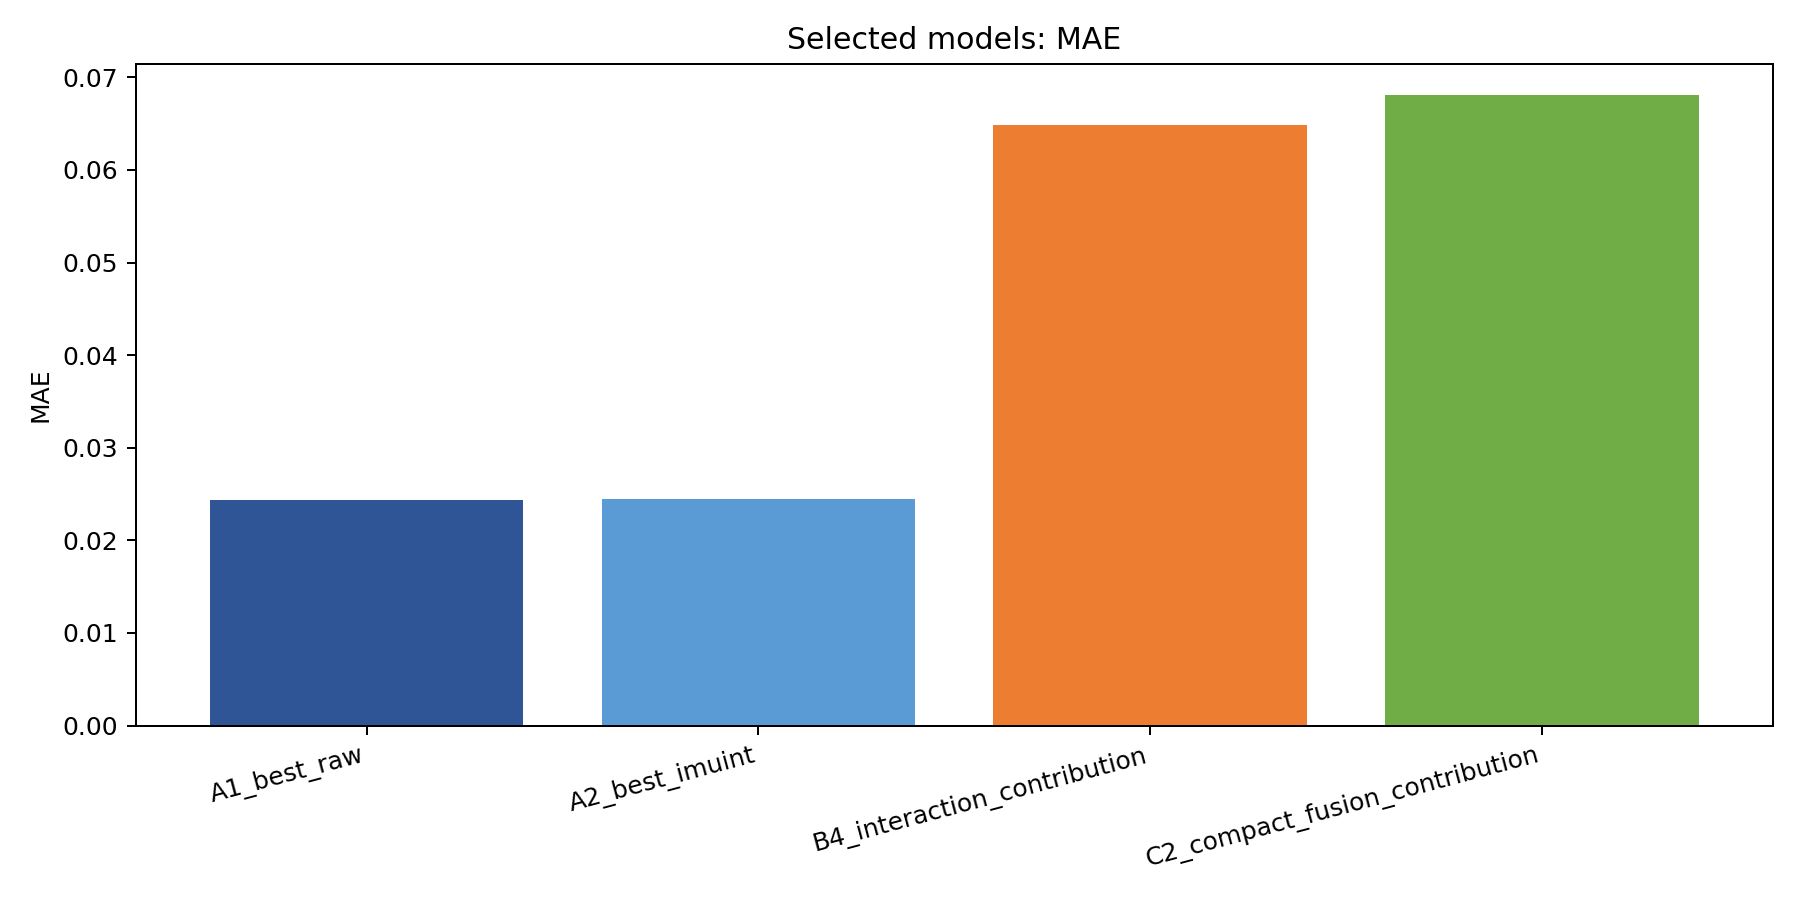
\includegraphics[width=0.85\linewidth]{selected_models_mae.png}
\caption{MAE comparison for the four selected models.}
\end{figure}

\begin{figure}[H]
\centering
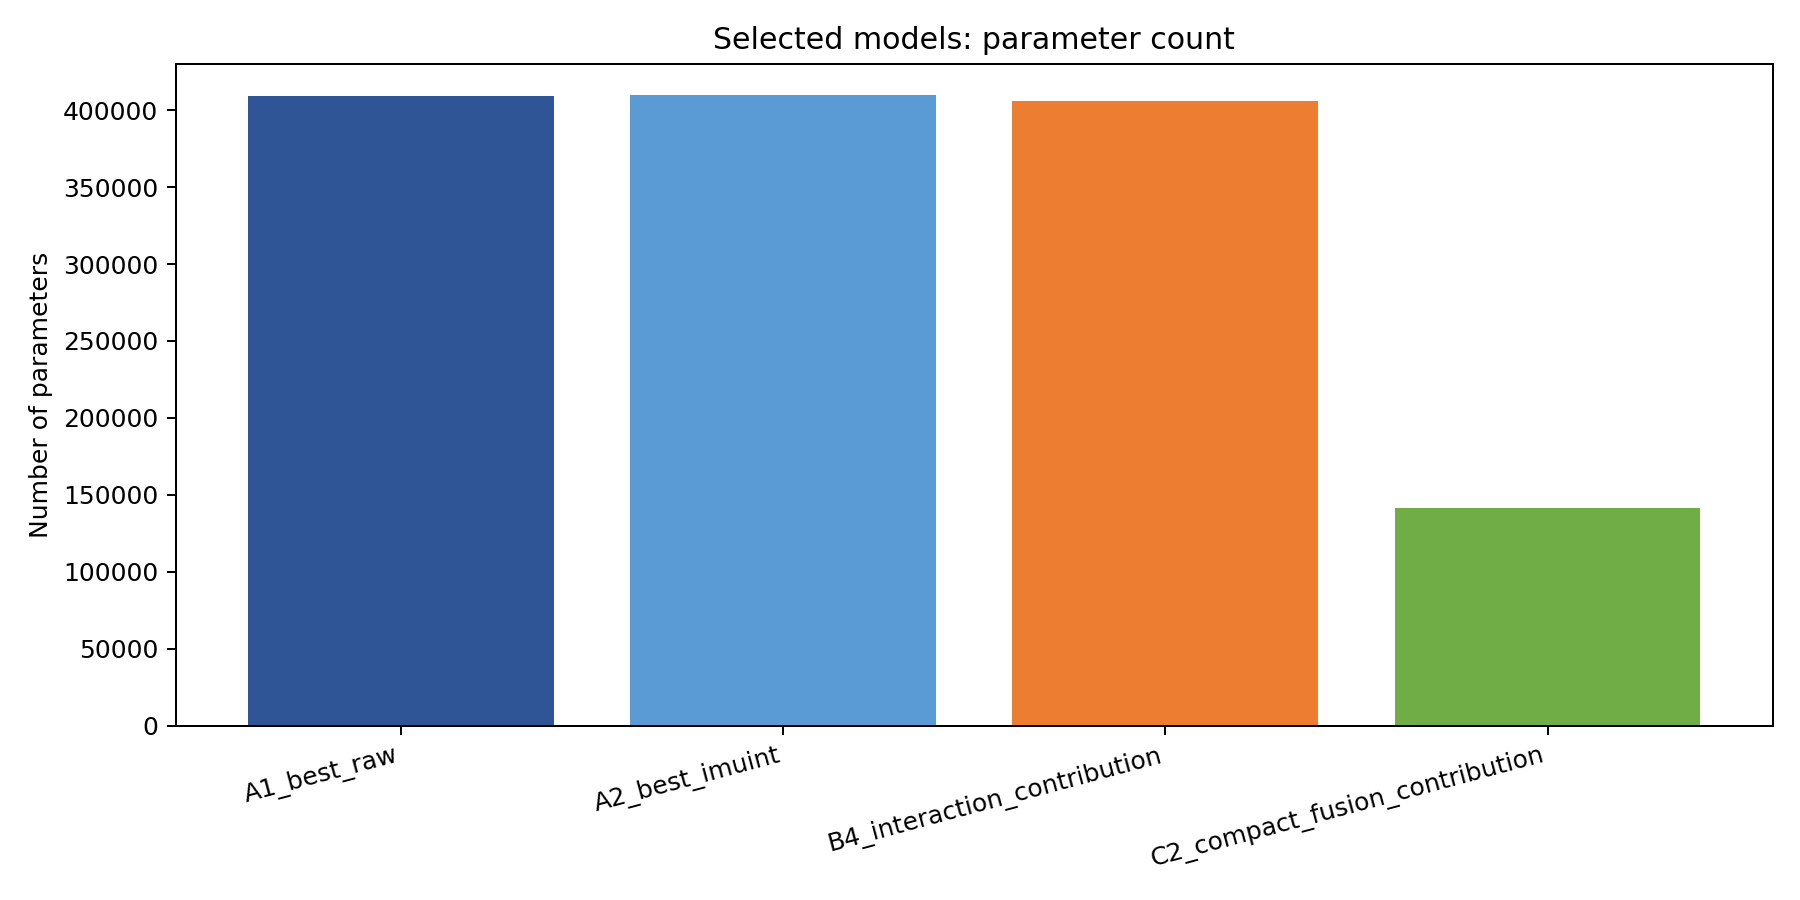
\includegraphics[width=0.85\linewidth]{selected_models_params.png}
\caption{Parameter count comparison. C2 is dramatically smaller than the other three models.}
\end{figure}

\begin{figure}[H]
\centering
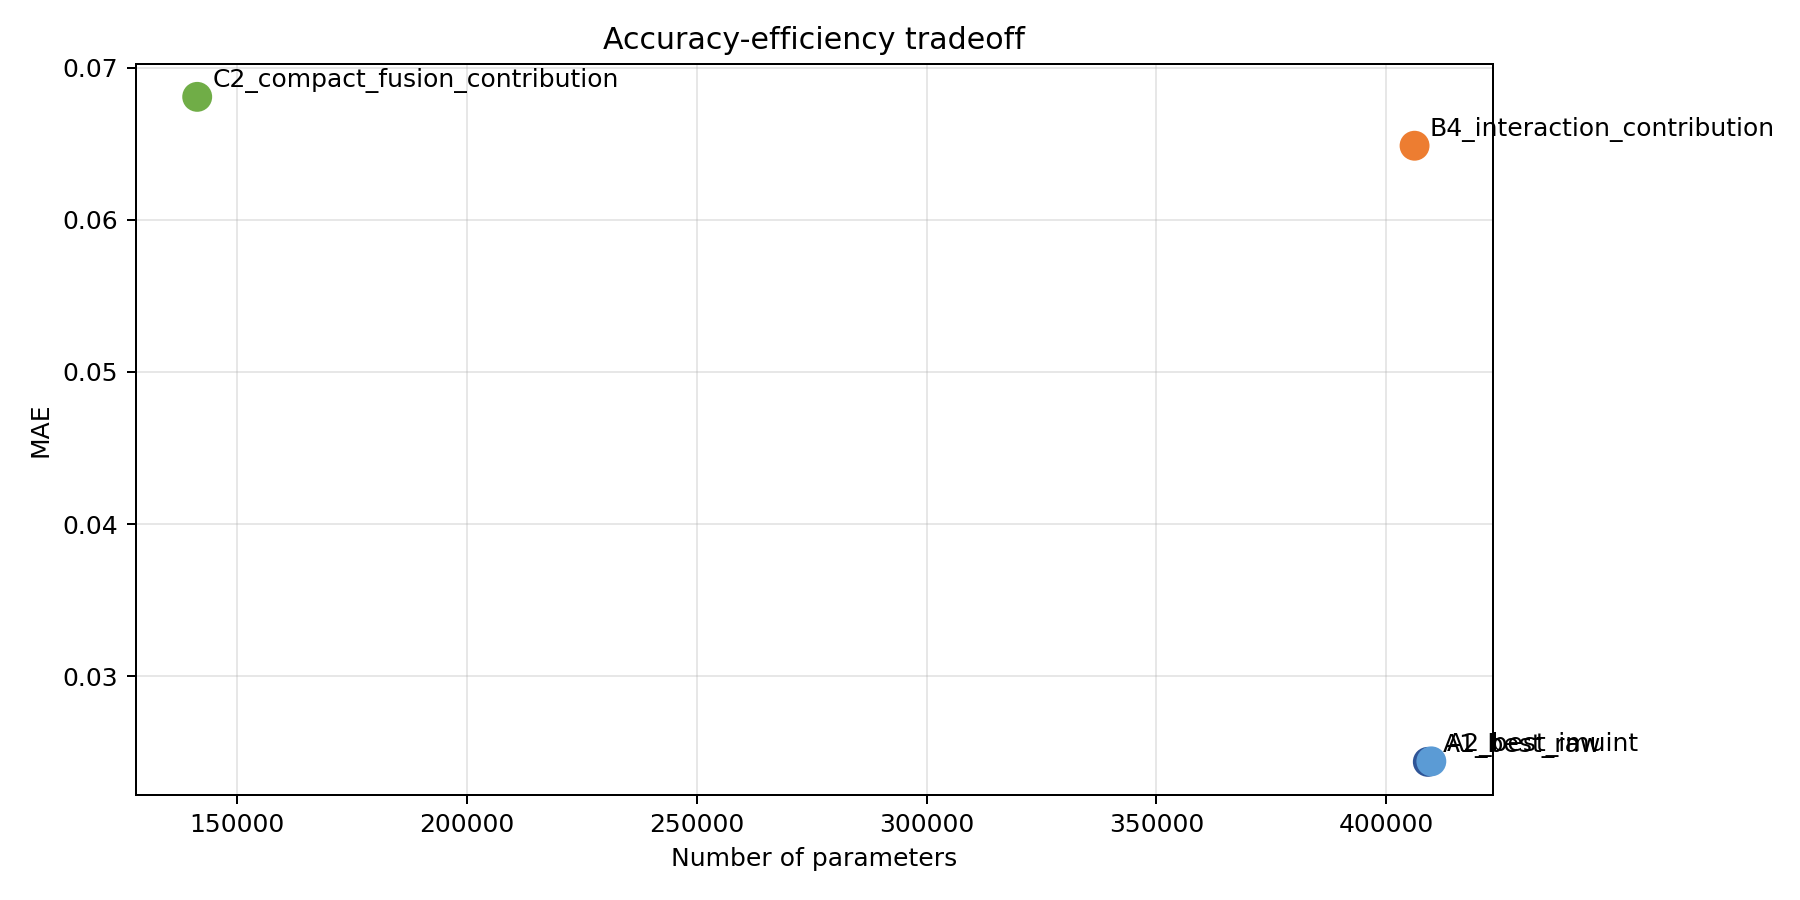
\includegraphics[width=0.85\linewidth]{selected_models_pareto.png}
\caption{Accuracy-efficiency tradeoff. A1 and A2 define the best-performance frontier; C2 defines the compact causal frontier.}
\end{figure}

\section{Detailed Input Feature Construction}

\subsection{A1\_best\_raw}

\textbf{Input groups:}
\begin{itemize}
\item mocap joint angles, velocities, accelerations: 18 channels
\item raw trunk IMU proxy channels (\texttt{roll}, \texttt{pitch}, \texttt{yaw}, \texttt{vel\_forward}): 4 channels
\item left/right exoskeleton torque: 2 channels
\item left/right GRF + contact: 8 channels
\item subject height/weight: 2 channels
\end{itemize}

Total input dimension: 34.

This model is best understood as the strongest privileged raw-feature baseline under the corrected target.
Its IMU block is still close to the earlier season1/season2 representation, and it keeps the full kinematic and GRF context.

\subsection{A2\_best\_imuint}

\textbf{Input groups:}
\begin{itemize}
\item mocap joint angles, velocities, accelerations: 18 channels
\item body-frame IMU: 7 channels
\item \texttt{imu\_integrated\_speed}: 1 channel
\item left/right exoskeleton torque: 2 channels
\item left/right GRF + contact: 8 channels
\item subject height/weight: 2 channels
\end{itemize}

Total input dimension: 38.

The key distinction from A1 is the inertial representation:
raw orientation-style IMU channels are replaced by a body-frame-aligned inertial representation plus a physically motivated speed prior obtained from leaky integration of overground-equivalent forward acceleration.

\subsection{B4\_interaction\_contribution}

\textbf{Input groups:}
\begin{itemize}
\item body-frame IMU: 7 channels
\item left/right robot hip angle, thigh angle, torque: 6 channels
\item interaction mechanics (\texttt{interaction\_power\_l/r}, \texttt{interaction\_work\_pos/neg}): 4 channels
\item subject height/weight: 2 channels
\end{itemize}

Total input dimension: 19.

This model intentionally removes privileged mocap and GRF. The contribution is not that it beats the teachers, but that it turns the problem into a deployable one while adding a mechanically meaningful prior: human-robot interaction power and accumulated work.

\subsection{C2\_compact\_fusion\_contribution}

\textbf{Input groups:}
\begin{itemize}
\item body-frame IMU: 7 channels
\item left/right robot hip angle, thigh angle, torque: 6 channels
\item \texttt{imu\_speed\_causal}: 1 channel
\item \texttt{stride\_speed\_robot}: 1 channel
\item interaction mechanics: 4 channels
\item subject height/weight: 2 channels
\end{itemize}

Total input dimension: 21.

This model is a compact structured-fusion system. It combines two causal priors:
\begin{itemize}
\item \texttt{imu\_speed\_causal}: a treadmill-independent inertial prior created by integrating body-frame forward acceleration without treadmill acceleration compensation
\item \texttt{stride\_speed\_robot}: a causal progression prior built from the phase difference and cadence proxy of left/right robot hip motion
\end{itemize}

On top of those, it uses a \texttt{FusionTCN\_GRU} head that learns confidence-like weights over the neural branch and the two priors.

\section{How the Contribution Features are Generated}

\subsection{Body-frame IMU}

Body-frame IMU is generated from the trunk IMU quaternion and raw local IMU measurements.
Acceleration and gyroscope are projected into a body-aligned right-forward-up frame.
The most task-relevant derived channel is \texttt{forward\_accel\_overground}, which approximates forward overground acceleration.

\subsection{IMU-integrated speed}

\texttt{imu\_integrated\_speed} is derived from body-frame forward acceleration using a causal leaky integration path.
This feature already performed strongly in season2 and remains highly competitive under the corrected target.

\subsection{Interaction power and work}

For each side, hip angular velocity is computed causally from exoskeleton hip angle using a backward difference and a causal low-pass filter.
Instantaneous power is:

\[
P_{\mathrm{side}}(t) = \tau_{\mathrm{side}}(t)\,\omega_{\mathrm{side}}(t)
\]

Positive and negative work are then tracked through exponentially weighted accumulation.
These features encode whether the exoskeleton is currently injecting or dissipating mechanical energy.

\subsection{Stride progression prior}

The stride progression prior uses the difference between left and right hip angle trajectories.
The magnitude of the phase difference acts as a stride excursion proxy, and the causal derivative magnitude acts as a cadence proxy.
The resulting product is low-pass filtered to produce a low-frequency progression-speed prior that is intended to align with the corrected speed target.

\section{Architecture Details}

\subsection{A1 and A2: TCN\_GRU teachers}

A1 and A2 both use the same backbone class: \texttt{TCN\_GRU}.
The architecture is:
\begin{itemize}
\item causal TCN encoder with channels \([32,32,64,64,128,128]\)
\item kernel size \(= 5\)
\item batch normalization in the TCN blocks
\item instance normalization on the input
\item GRU head with hidden size 32
\item linear output head
\end{itemize}

The difference between A1 and A2 is therefore almost entirely in the \emph{input representation}, not in the model class itself.
This makes their near-identical performance especially informative: it means both feature formulations are highly competitive under the corrected target.

\subsection{B4: deployable causal baseline}

B4 also uses \texttt{TCN\_GRU} with the same channel width as A1/A2.
Its importance is therefore not architectural novelty but \emph{signal design novelty}.
It asks a direct question:

\begin{quote}
How much of the corrected progression-speed target can we recover using only deployable causal measurements and interaction-aware mechanics?
\end{quote}

\subsection{C2: compact FusionTCN\_GRU}

C2 uses \texttt{FusionTCN\_GRU} with smaller channel widths:
\([24,24,48,48,64,64]\), GRU hidden size 24, window size 150, and fusion priors on channels 13 and 14.

The fusion head constructs three sources:
\begin{itemize}
\item learned network prediction
\item \texttt{imu\_speed\_causal}
\item \texttt{stride\_speed\_robot}
\end{itemize}

It then learns source weights through a softmax over fusion logits.
This turns the final estimate into a confidence-weighted combination of the neural branch and two causal priors.

\section{Quantitative Analysis}

\subsection{Best-performance models}

A1 and A2 are effectively tied:
\begin{itemize}
\item A1 beats A2 in MAE by only \(3.29 \times 10^{-5}\)
\item A2 is slightly faster in host latency
\item the parameter difference is negligible
\end{itemize}

That result is scientifically useful.
It shows that, under the corrected target, replacing raw trunk IMU channels with body-frame IMU plus \texttt{imu\_integrated\_speed} does not create a dramatic numerical gain, but it also does not harm the upper bound.
In other words, both signal representations remain defensible top-performing teacher choices.

\subsection{Contribution models}

B4 and C2 should not be judged only by raw MAE.

\paragraph{B4}
\begin{itemize}
\item preserves a standard TCN\_GRU capacity
\item removes mocap and GRF
\item uses only deployable causal features
\item introduces interaction power/work as a biomechanics-aware contribution
\end{itemize}

\paragraph{C2}
\begin{itemize}
\item keeps deployment-side feature design
\item introduces structured multi-prior fusion
\item uses a shorter window (150 vs. 200)
\item reduces parameters from 409,025 to 141,381
\end{itemize}

Relative to A1:
\begin{itemize}
\item C2 keeps only \(34.6\%\) of the parameters
\item equivalently, it reduces parameter count by \(65.4\%\)
\item MAE rises from 0.02439 to 0.06808
\end{itemize}

Relative to B4:
\begin{itemize}
\item C2 is only slightly worse in MAE (0.06808 vs. 0.06486)
\item C2 is much smaller in parameter count
\item therefore C2 is the stronger efficiency-focused paper candidate
\end{itemize}

\section{Qualitative Plot Analysis}

\subsection{A1 and A2}

\begin{figure}[H]
\centering
\begin{minipage}{0.49\linewidth}
\centering
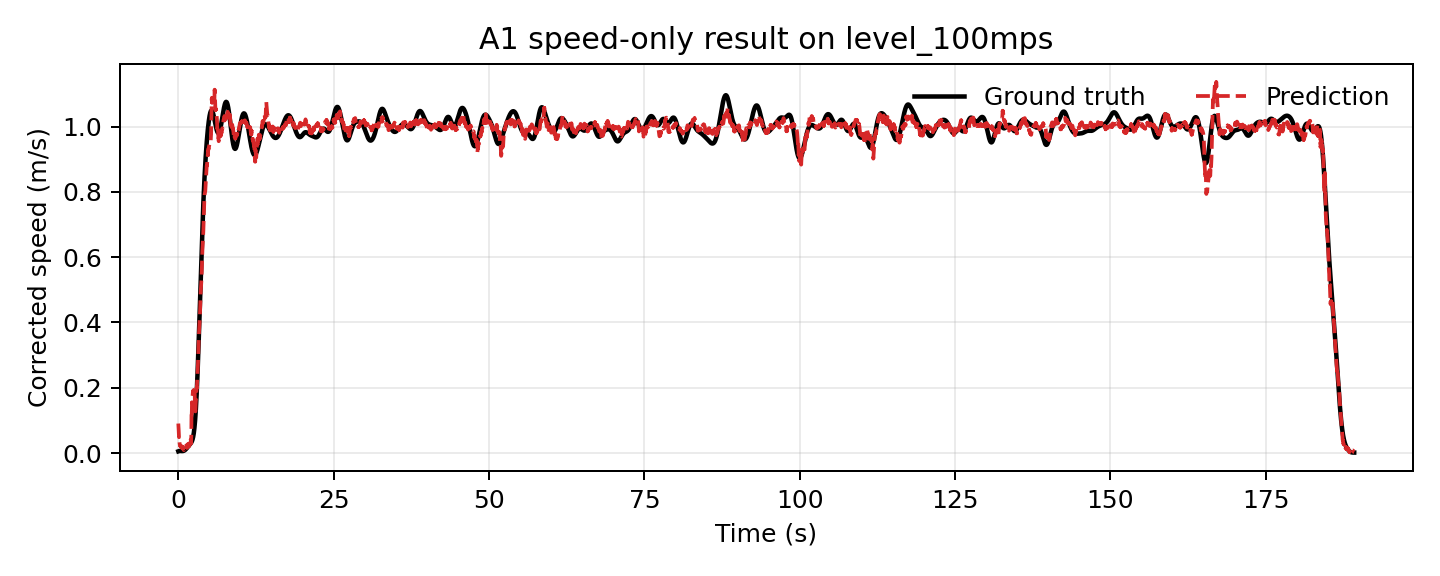
\includegraphics[width=\linewidth]{A1_speed_level100.png}\\
\small A1 on level\_100mps
\end{minipage}
\hfill
\begin{minipage}{0.49\linewidth}
\centering
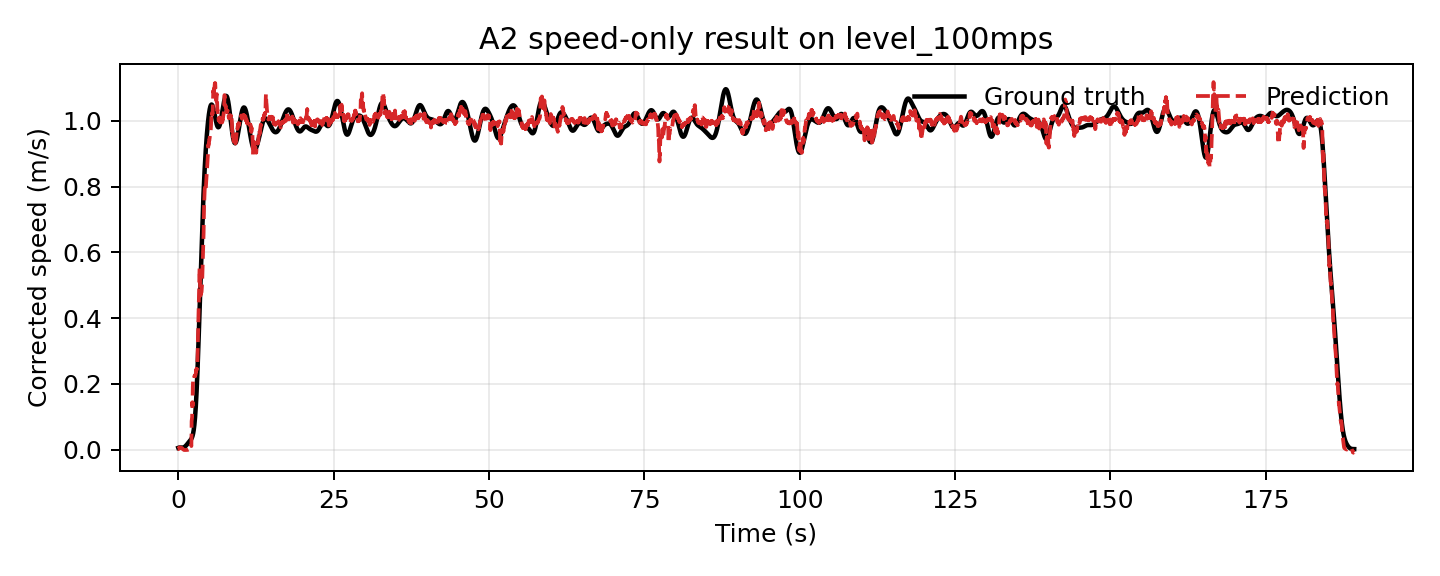
\includegraphics[width=\linewidth]{A2_speed_level100.png}\\
\small A2 on level\_100mps
\end{minipage}
\caption{Best-performance models on a constant-speed condition.}
\end{figure}

\begin{figure}[H]
\centering
\begin{minipage}{0.49\linewidth}
\centering
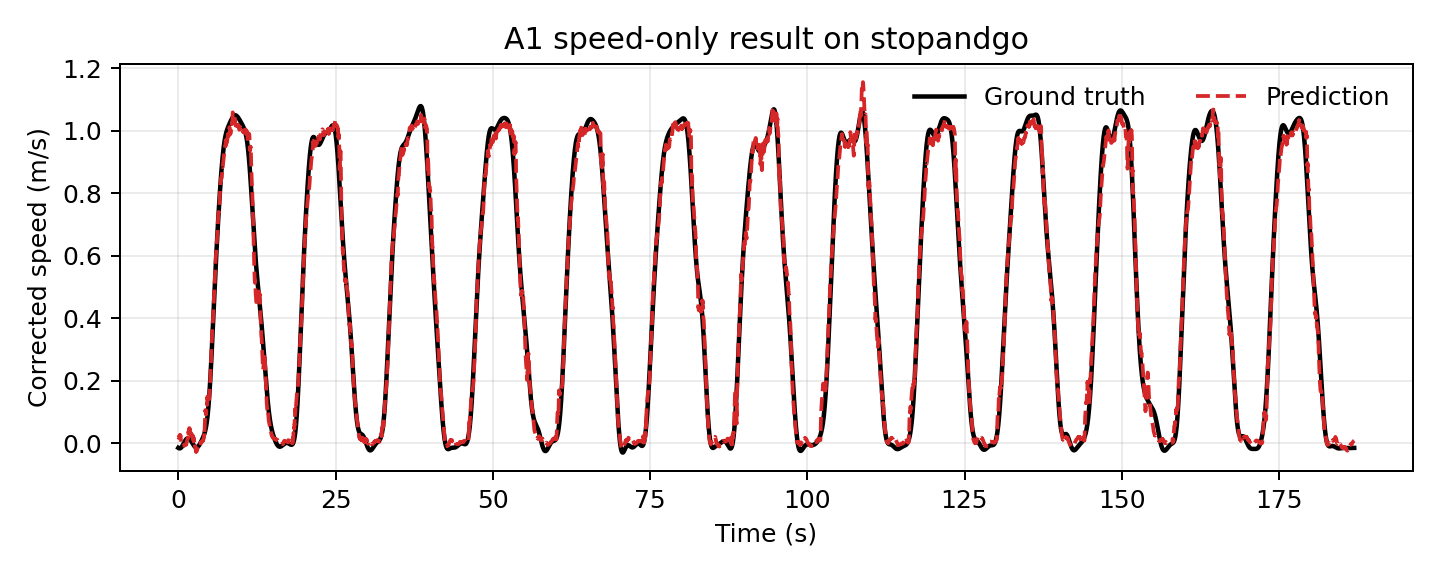
\includegraphics[width=\linewidth]{A1_speed_stopandgo.png}\\
\small A1 on stopandgo
\end{minipage}
\hfill
\begin{minipage}{0.49\linewidth}
\centering
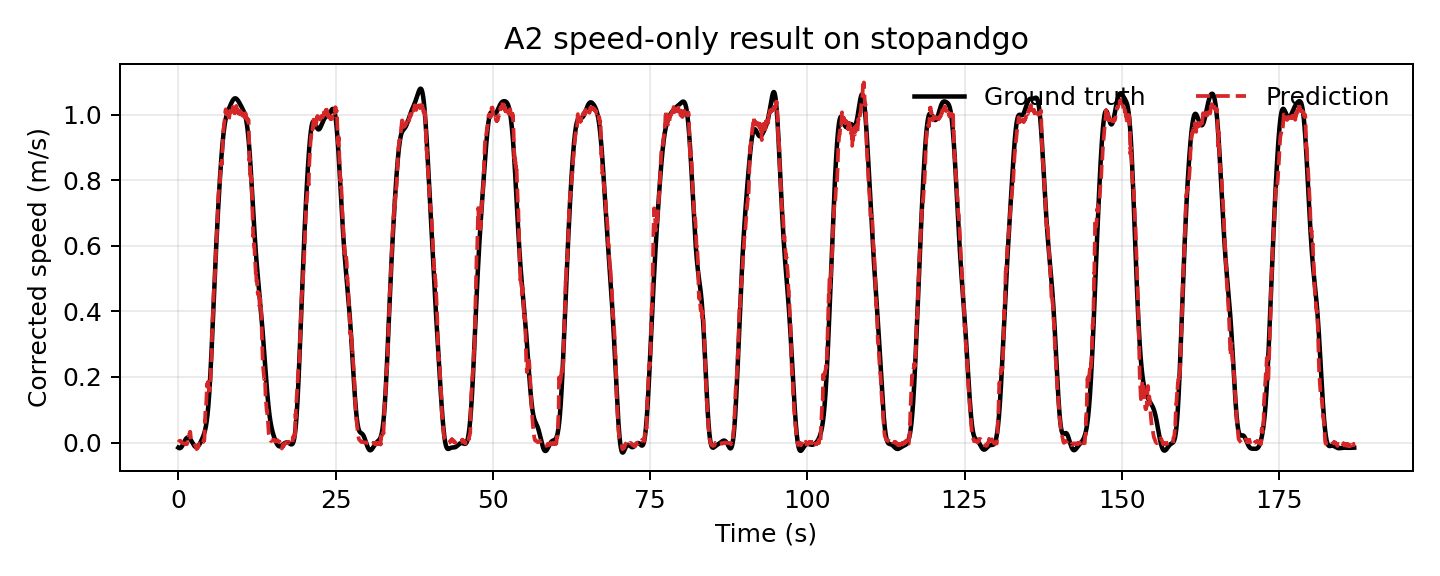
\includegraphics[width=\linewidth]{A2_speed_stopandgo.png}\\
\small A2 on stopandgo
\end{minipage}
\caption{Best-performance models on a transition-heavy condition.}
\end{figure}

The qualitative behavior of A1 and A2 is consistent with their nearly identical metrics.
Both track the corrected speed target well in level walking and remain comparatively stable through stop-and-go transitions.
A2 often appears slightly smoother because of the body-frame inertial prior, while A1 remains very competitive through its privileged raw feature set.

\begin{figure}[H]
\centering
\begin{minipage}{0.49\linewidth}
\centering
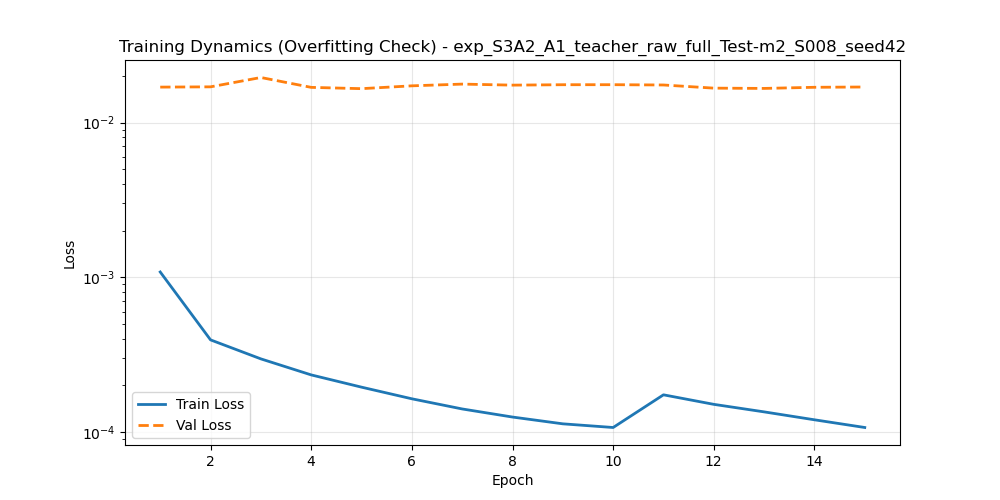
\includegraphics[width=\linewidth]{A1_training_curves.png}\\
\small A1 training curve
\end{minipage}
\hfill
\begin{minipage}{0.49\linewidth}
\centering
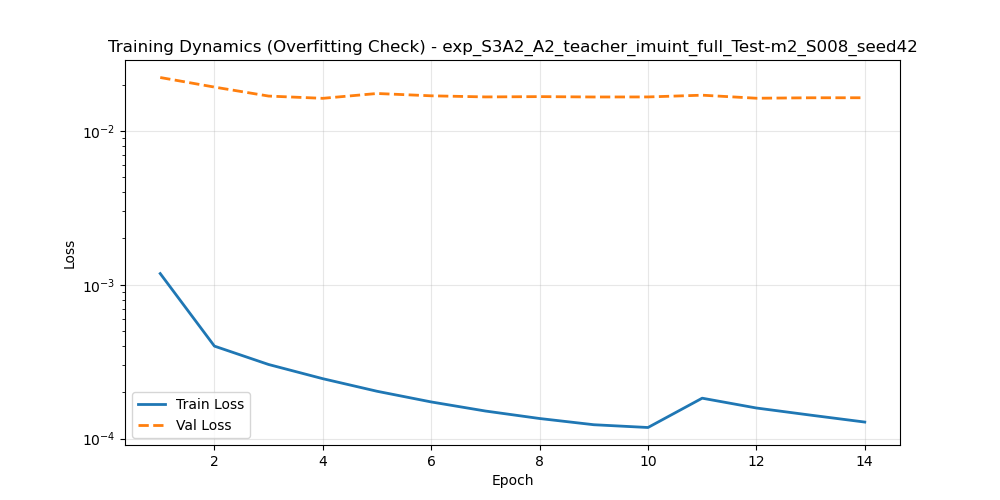
\includegraphics[width=\linewidth]{A2_training_curves.png}\\
\small A2 training curve
\end{minipage}
\caption{Training curves for the two best-performing models.}
\end{figure}

\subsection{B4 and C2}

\begin{figure}[H]
\centering
\begin{minipage}{0.49\linewidth}
\centering
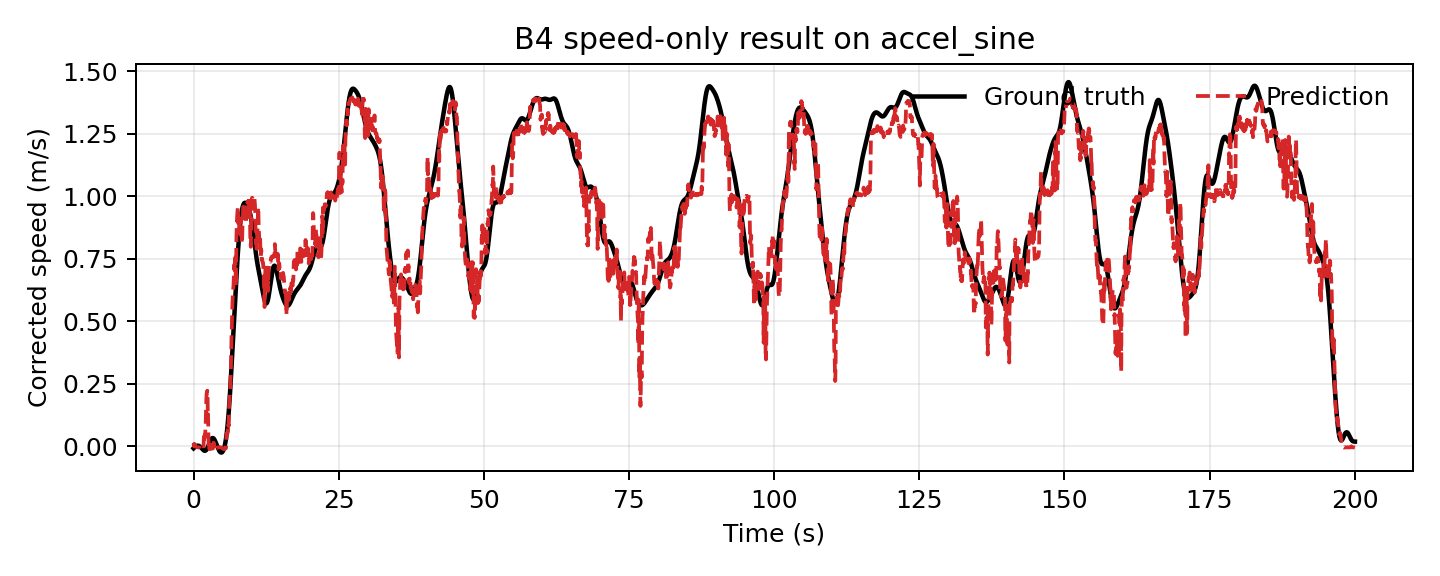
\includegraphics[width=\linewidth]{B4_speed_accelsine.png}\\
\small B4 on accel\_sine
\end{minipage}
\hfill
\begin{minipage}{0.49\linewidth}
\centering
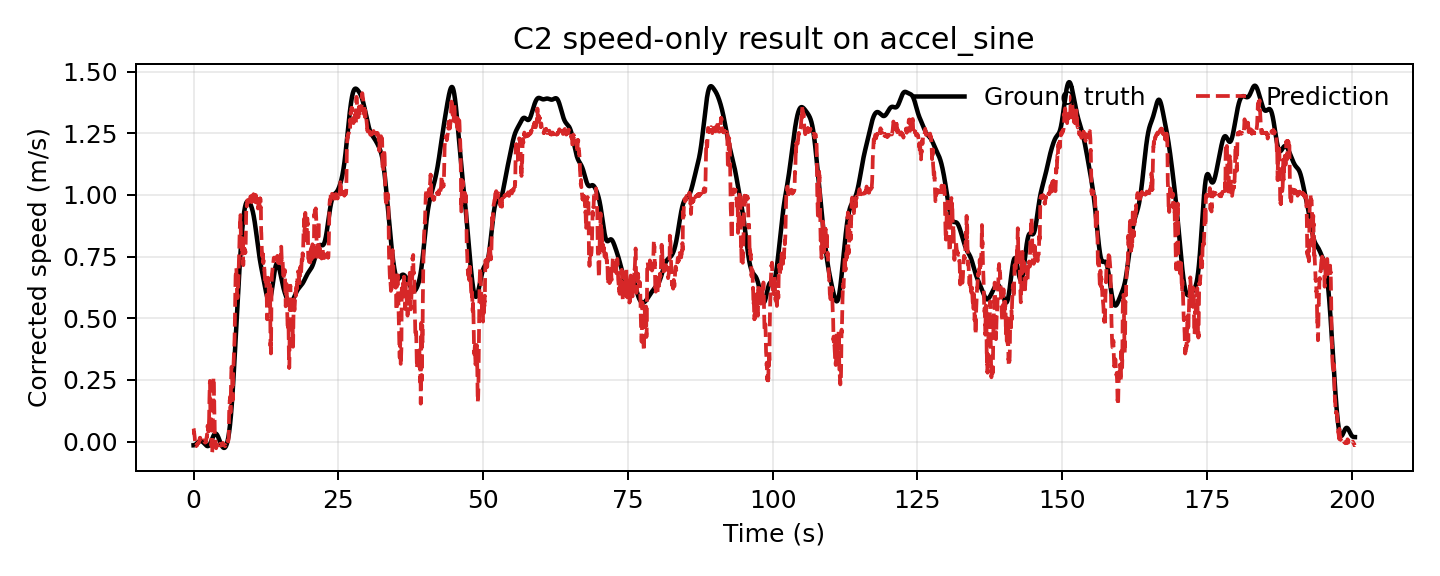
\includegraphics[width=\linewidth]{C2_speed_accelsine.png}\\
\small C2 on accel\_sine
\end{minipage}
\caption{Contribution models on a continuously varying-speed condition.}
\end{figure}

\begin{figure}[H]
\centering
\begin{minipage}{0.49\linewidth}
\centering
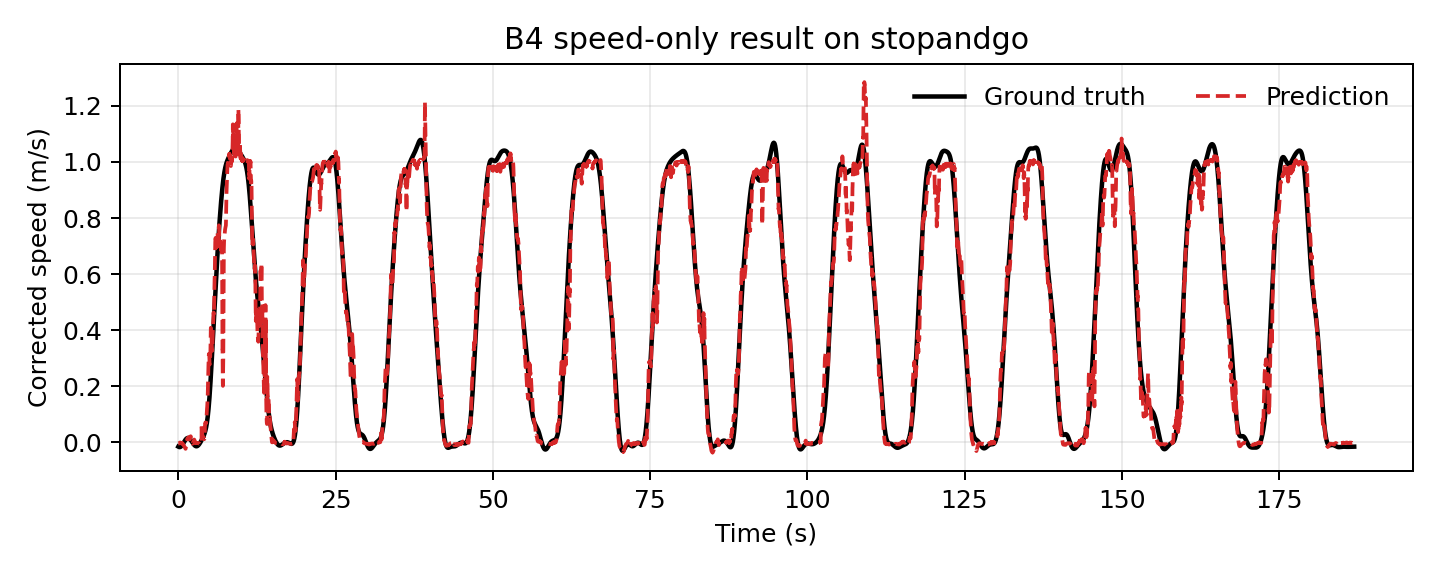
\includegraphics[width=\linewidth]{B4_speed_stopandgo.png}\\
\small B4 on stopandgo
\end{minipage}
\hfill
\begin{minipage}{0.49\linewidth}
\centering
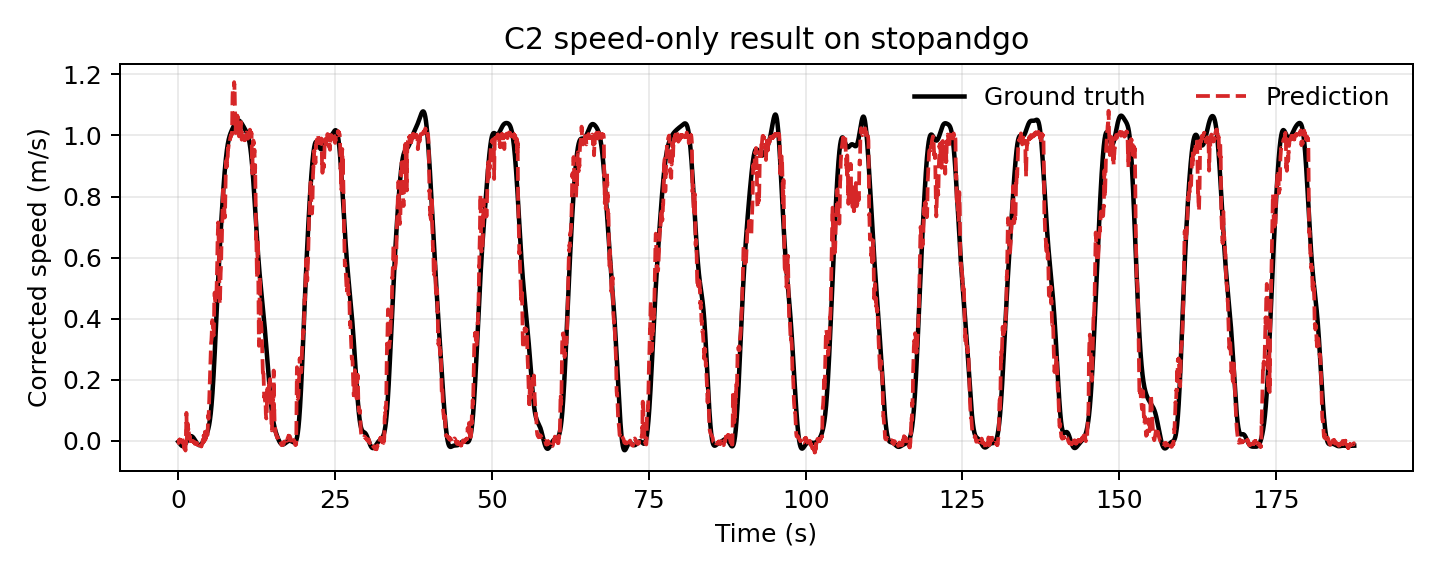
\includegraphics[width=\linewidth]{C2_speed_stopandgo.png}\\
\small C2 on stopandgo
\end{minipage}
\caption{Contribution models on a difficult transition condition.}
\end{figure}

\begin{figure}[H]
\centering
\begin{minipage}{0.49\linewidth}
\centering
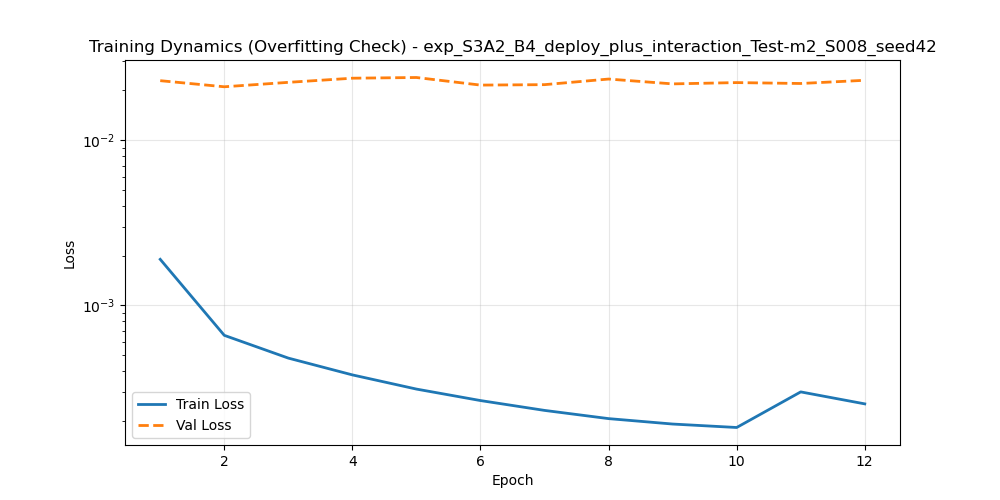
\includegraphics[width=\linewidth]{B4_training_curves.png}\\
\small B4 training curve
\end{minipage}
\hfill
\begin{minipage}{0.49\linewidth}
\centering
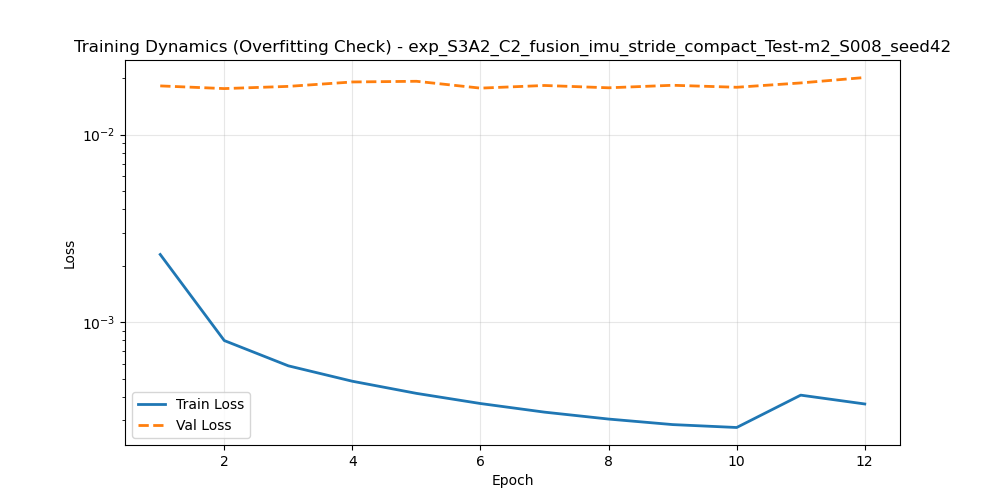
\includegraphics[width=\linewidth]{C2_training_curves.png}\\
\small C2 training curve
\end{minipage}
\caption{Training curves for the two contribution-heavy models.}
\end{figure}

Qualitatively, B4 and C2 are naturally less precise than A1 and A2.
That is expected because they intentionally give up privileged sensors.
The important observation is not absolute superiority, but that they retain meaningful target tracking while respecting the project's causal and deployable input rules.

\section{Feature Importance}

The following plots show sampled permutation importance on held-out windows.
Higher values mean that permuting the feature increases MAE more strongly.

\subsection{A1\_best\_raw}

\begin{figure}[H]
\centering
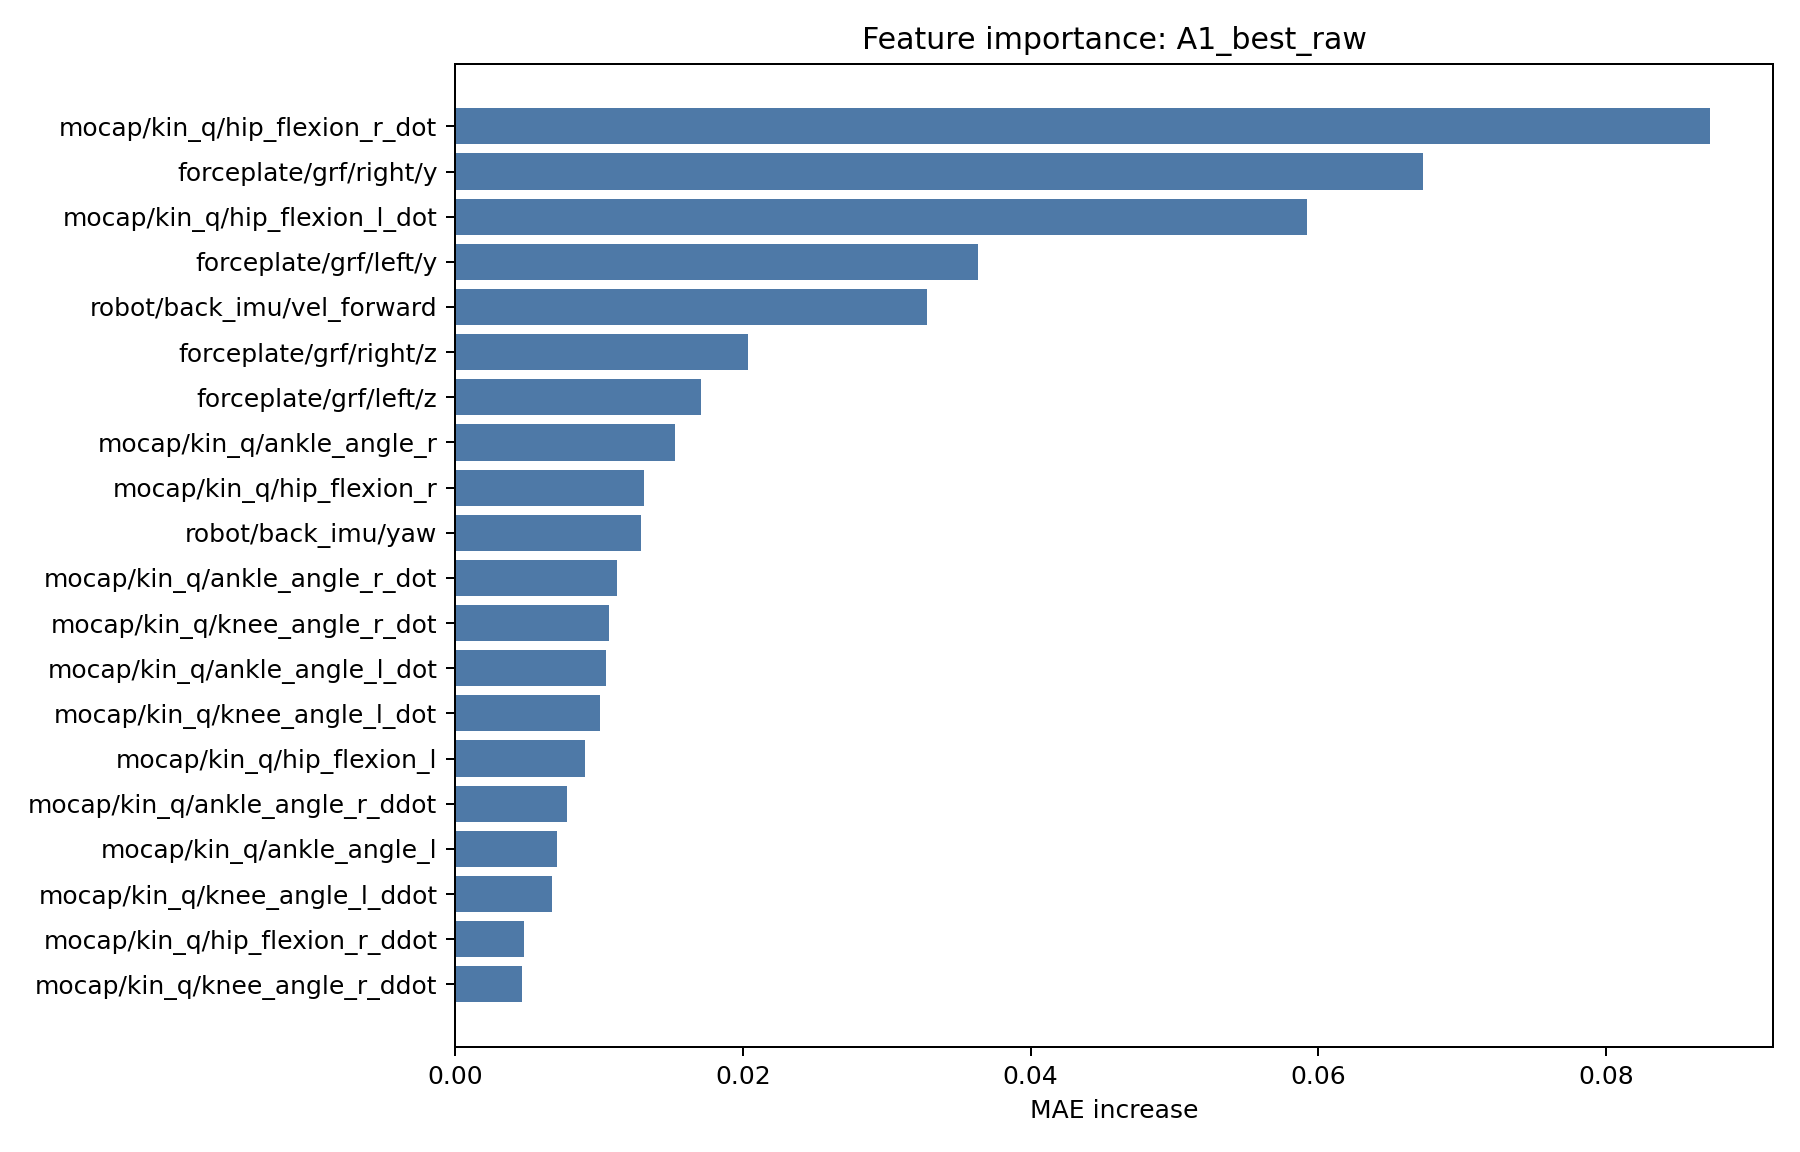
\includegraphics[width=0.82\linewidth]{A1_best_raw_feature_importance_top20.png}
\caption{Sampled permutation importance for A1\_best\_raw.}
\end{figure}

For A1, the dominant features are hip angular velocities, GRF channels, and the raw forward-velocity proxy from trunk IMU.
This matches the model's design: it wins by leveraging privileged biomechanical observability, especially kinematics and force information.

\subsection{A2\_best\_imuint}

\begin{figure}[H]
\centering
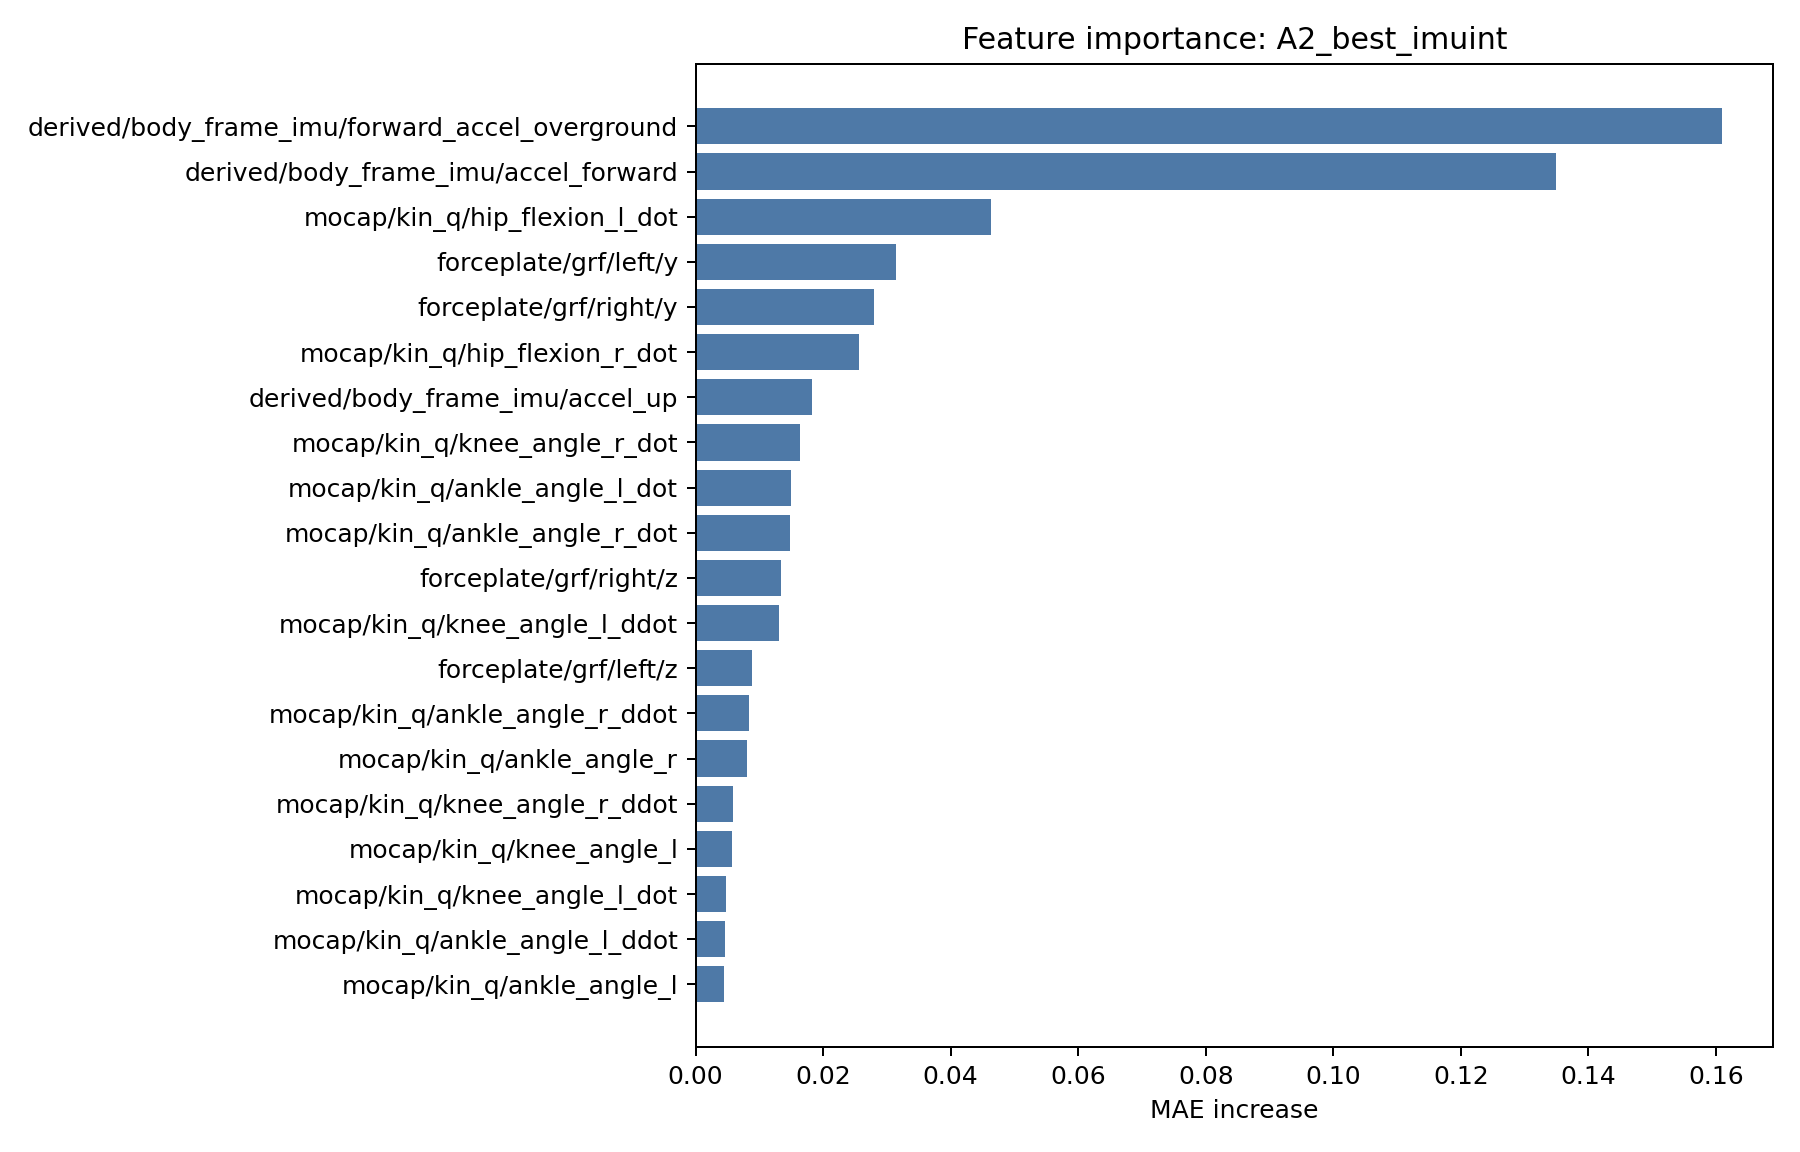
\includegraphics[width=0.82\linewidth]{A2_best_imuint_feature_importance_top20.png}
\caption{Sampled permutation importance for A2\_best\_imuint.}
\end{figure}

For A2, the expected interpretation is that body-frame inertial channels and the IMU-integrated speed prior rise in importance relative to A1's raw trunk IMU representation.
That is exactly what appears in the sampled importance ranking:
\texttt{forward\_accel\_overground} and \texttt{accel\_forward} dominate the list, followed by hip angular velocities and GRF channels.
This supports the claim that A2 is the cleaner inertial upper-bound model.

\subsection{B4\_interaction\_contribution}

\begin{figure}[H]
\centering
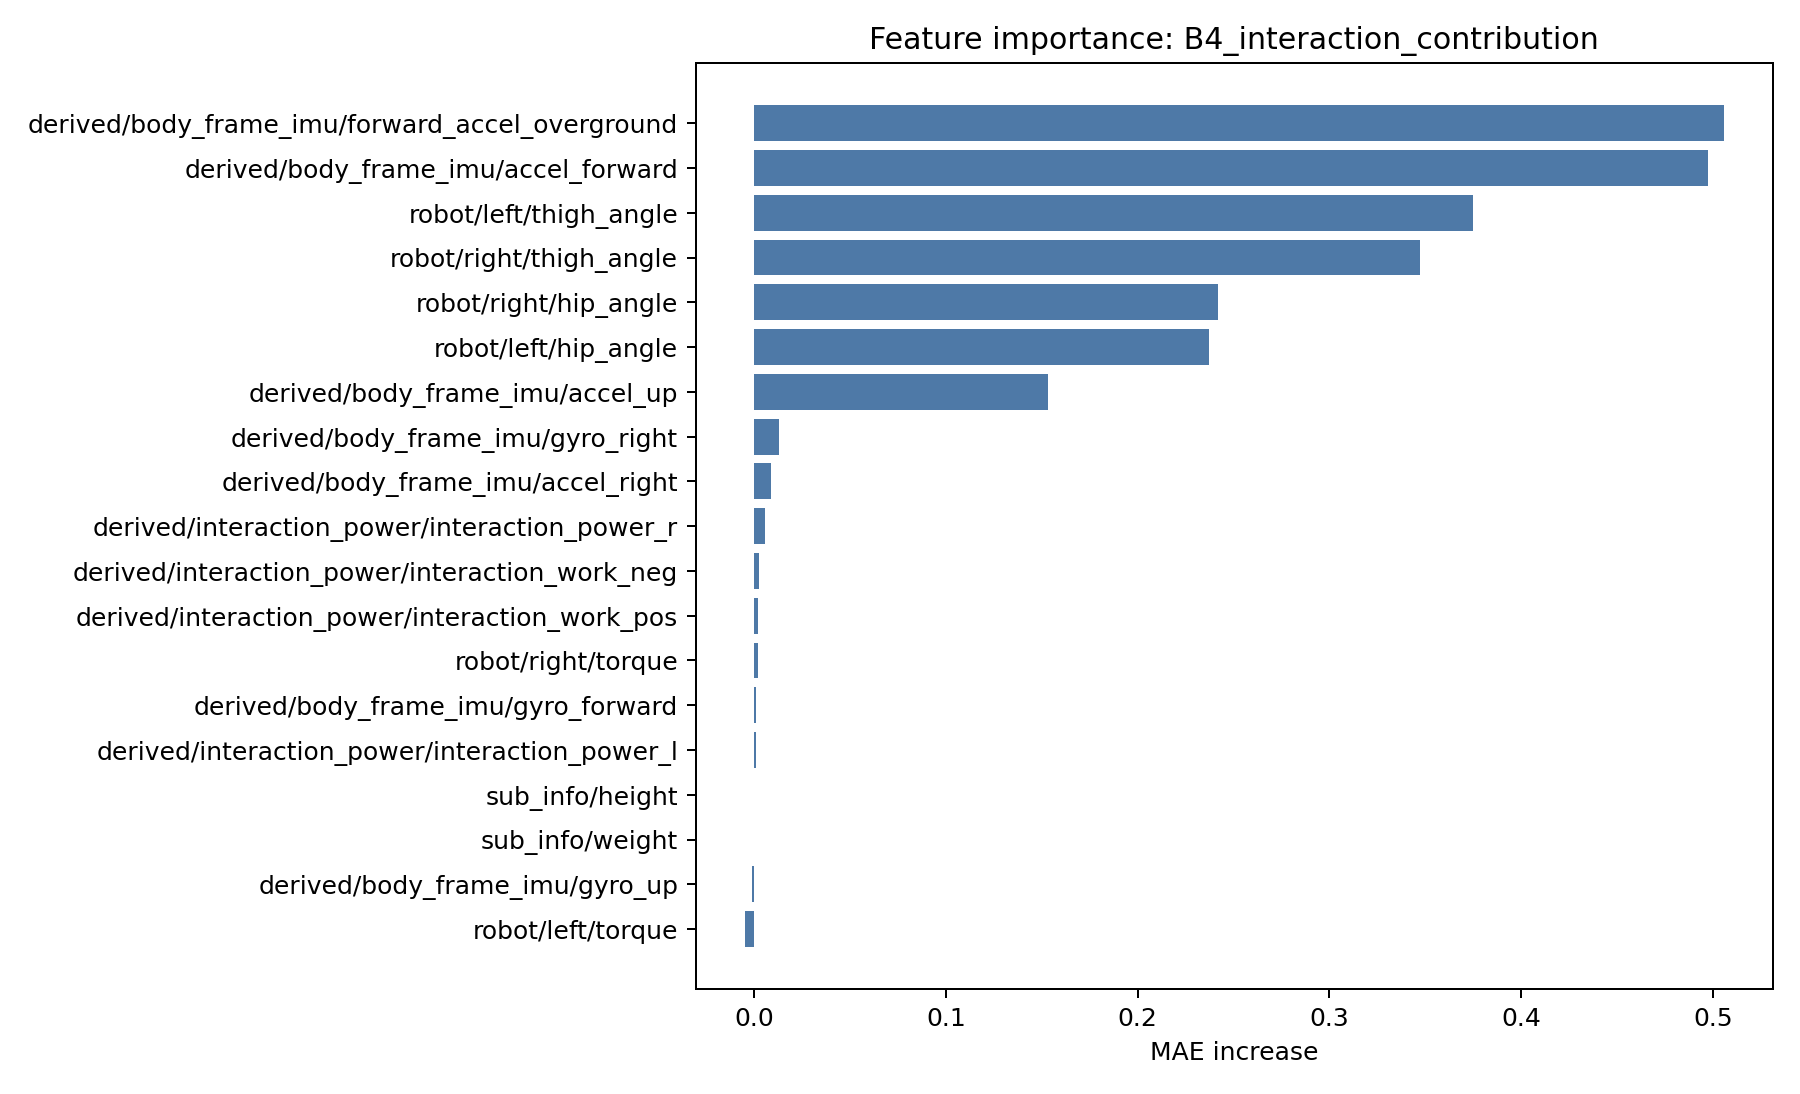
\includegraphics[width=0.82\linewidth]{B4_interaction_contribution_feature_importance_top20.png}
\caption{Sampled permutation importance for B4\_interaction\_contribution.}
\end{figure}

This plot is central for the contribution claim.
The honest reading is nuanced:
the dominant channels are still body-frame forward and upward acceleration together with robot thigh/hip angles.
The interaction channels are \emph{not} the top-ranked features overall, but \texttt{interaction\_power\_r} and \texttt{interaction\_work\_neg} do appear among the informative channels.
That means the interaction mechanics are contributing, but as a secondary cue that complements inertial and joint-angle information rather than replacing it.

\subsection{C2\_compact\_fusion\_contribution}

\begin{figure}[H]
\centering
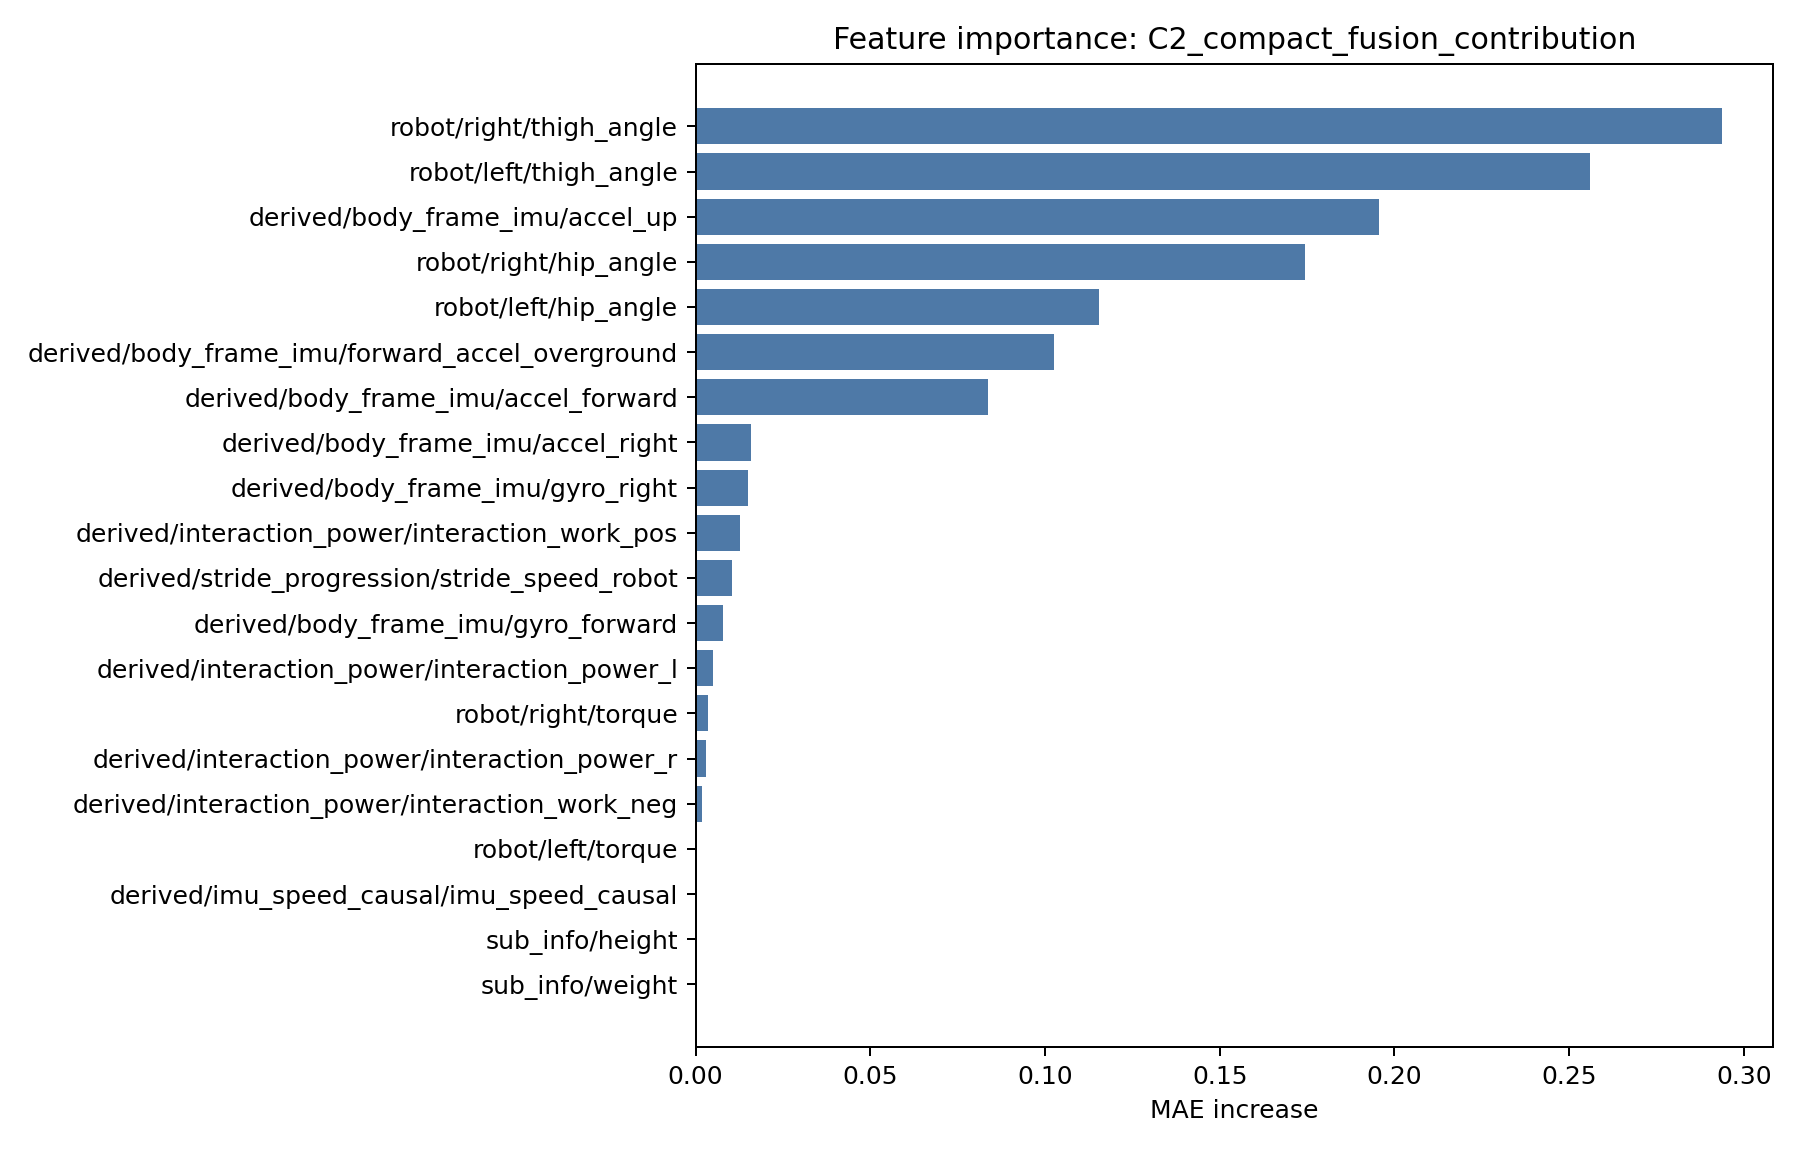
\includegraphics[width=0.82\linewidth]{C2_compact_fusion_contribution_feature_importance_top20.png}
\caption{Sampled permutation importance for C2\_compact\_fusion\_contribution.}
\end{figure}

For C2, the sampled ranking shows that the model still leans most heavily on robot thigh/hip angles and body-frame acceleration channels.
The explicit priors are present but secondary:
\texttt{stride\_speed\_robot} appears in the informative set, while the causal IMU prior is less dominant than the kinematic and inertial channels.
This is still useful for the paper story.
It means the compact fusion architecture is not winning purely because of the priors; rather, it uses a strong causal motion representation and benefits from prior-guided fusion as a stabilizing structural bias.

\section{Paper Interpretation}

\subsection{What the paper should claim}

The safest and strongest paper framing is:

\begin{quote}
We estimate a corrected progression-speed state under strict causal/deployable input constraints, and we characterize the gap between privileged upper-bound models and deployable structured-prior models.
\end{quote}

This lets the paper claim:
\begin{itemize}
\item a corrected and physically better-grounded target definition
\item clear separation between upper-bound and deployable models
\item causal deployable biomechanical priors
\item an interaction-aware deployable model (B4)
\item a compact structured-fusion model with large parameter reduction (C2)
\end{itemize}

\subsection{What the paper should not claim}

The paper should \emph{not} claim that B4 or C2 are the overall best models.
They are not. A1 and A2 are better in MAE.

The paper should instead claim:
\begin{itemize}
\item A1/A2 are the best-performing corrected-target upper bounds
\item B4 is the best contribution model for deployable biomechanics-aware feature design
\item C2 is the best contribution model for compact structured causal fusion
\end{itemize}

\section{Recommended Main Figures for the Paper}

If the paper needs a minimal but strong set of figures, the following should be prioritized:

\begin{enumerate}
\item MAE comparison across A1, A2, B4, C2
\item parameter-count comparison, highlighting the compactness of C2
\item A1 vs A2 qualitative plots on \texttt{level\_100mps} and \texttt{stopandgo}
\item B4 vs C2 qualitative plots on \texttt{accel\_sine} and \texttt{stopandgo}
\item feature importance for B4 and C2
\end{enumerate}

Among these, the two most paper-critical are:
\begin{itemize}
\item B4 feature importance, because it validates the interaction-power contribution
\item the A1/C2 pareto comparison, because it quantifies the accuracy--efficiency tradeoff
\end{itemize}

\section{Limitations}

\begin{itemize}
\item The current comparison is still a single-LOSO result on \texttt{m2\_S008}, not a full-LOSO aggregate across all subjects.
\item The contribution models still show a large gap to the privileged upper bound.
\item B4 is deployable, but not compact.
\item C2 is compact and deployable, but not yet close to the A1/A2 accuracy level.
\item Distillation remains an open direction; the current distillation variants did not become top paper candidates.
\end{itemize}

\section{Final Recommendation}

If the paper needs four core models, the recommended usage is:

\begin{itemize}
\item \textbf{A1\_best\_raw}: report as the strongest corrected-target raw privileged baseline
\item \textbf{A2\_best\_imuint}: report as the strongest corrected-target inertial upper bound
\item \textbf{B4\_interaction\_contribution}: report as the primary deployable biomechanics-aware contribution model
\item \textbf{C2\_compact\_fusion\_contribution}: report as the primary compact structured-fusion contribution model
\end{itemize}

This gives the paper a balanced narrative:
\begin{itemize}
\item two models that establish what the task can achieve with strong sensing
\item two models that establish what can be deployed causally with a meaningful contribution story
\end{itemize}

\section*{Appendix: Model-by-Model Snapshot}

\small
\begin{longtable}{>{\raggedright\arraybackslash}p{1.3cm} >{\raggedright\arraybackslash}p{4.2cm} >{\raggedright\arraybackslash}p{3.7cm} >{\raggedright\arraybackslash}p{4.0cm}}
\toprule
Model & Input summary & Model summary & Main interpretation \\
\midrule
\endhead

\texttt{A1} &
18 kinematic channels, 4 raw trunk IMU channels, 2 torques, 8 GRF/contact channels, 2 anthropometric channels &
TCN\_GRU, window 200, channels [32,32,64,64,128,128], GRU 32 &
Best corrected-target privileged raw baseline; strongest absolute MAE \\

\texttt{A2} &
18 kinematic channels, 7 body-frame IMU channels, 1 IMU-integrated speed prior, 2 torques, 8 GRF/contact channels, 2 anthropometric channels &
TCN\_GRU, window 200, channels [32,32,64,64,128,128], GRU 32 &
Best corrected-target inertial upper bound; validates body-frame plus inertial-speed representation \\

\texttt{B4} &
7 body-frame IMU channels, 6 robot kinematic/torque channels, 4 interaction power/work channels, 2 anthropometric channels &
TCN\_GRU, window 200, same width as teacher models &
Best deployable biomechanics-aware signal-design contribution; removes privileged mocap and GRF \\

\texttt{C2} &
7 body-frame IMU channels, 6 robot kinematic/torque channels, 1 causal IMU prior, 1 stride prior, 4 interaction channels, 2 anthropometric channels &
FusionTCN\_GRU, window 150, compact width [24,24,48,48,64,64], GRU 24 &
Best compact deployable contribution; structured fusion of two causal priors with major parameter reduction \\

\bottomrule
\end{longtable}

\end{document}
